\documentclass[11pt,a4paper,DIV=10,]{scrartcl}
\usepackage[utf8]{inputenc}
\usepackage[ngerman]{babel}
\usepackage{amsmath}
\usepackage{amsfonts}
\usepackage{amssymb}
\usepackage{fancybox}
\usepackage{multicol}
\usepackage{graphicx}
\usepackage{color}
\usepackage{colortbl}
% Define user colors using the RGB model
\definecolor{dunkelgrau}{rgb}{0.8,0.8,0.8}
\definecolor{hellgrau}{rgb}{0.95,0.95,0.95}
\usepackage[normal,font={small,color=black}, labelfont=bf,figurename=Abb.]{caption}
\usepackage{float}
\usepackage{cite}
\usepackage{url}
\bibliographystyle{unsrtnat}
\usepackage[numbers]{natbib}
%\usepackage[T1]{fontenc}

\begin{document}
\onecolumn
\subsection*{ALP4 SoSe 2013, Di. 16-18}
\section*{Lösung Übungsblatt 1}
\textbf{Christoph van Heteren-Frese (Matr.-Nr.: 4465677), \\ Sven Wildermann (Matr.-Nr.: 4567553)}\\
Tutor: Alexander Steen, eingereicht am \today\\
\hrule

\section*{Aufgabe 1}
\subsection*{a)}
Diese Aussage ist richtig. Wenn die Reihenfolge der einzelnen Anweisungen eindeutig festgelegt ist (also deterministisch ist), so muss bei gleichen Eingabewerten trivialerweise auch der gleiche Ausgabewert (determiniert) geliefert  werden. 
\subsection*{b)}
Diese Aussage ist falsch. Nur weil das Ergebnis eines Algorithmusses bei gleichen Eingabewerten das selbe ist, muss die Reihenfolge der Anweisungen
nicht zwangsläufig die selbe sein. Beispiel: Das Ergebnis von zwei Additionen auf eine Variable X ist unabhängig davon welcher der beiden Additionen
zuerst ausgeführt wird. 
\subsection*{c)}
Diese Aussage stimmt, da die Sequenz eines deterministischen Algorithmus die Folge der Schritte seines Ablaufes ist. Andersherum ist da jedoch nicht der Fall. 
\subsection*{d)}
Diese Aussage ist falsch, da ein nichtsequentieller Algorithmus auch determiniert sein kann. 
Genau wie in b) kann das Ergebnis eines Algorithmusses bei gleichen Eingabewerten das selbe sein, auch wenn die Reihenfolge der Anweisungen
nicht zwangsläufig die selbe sein. Beispiel: Das Ergebnis von zwei Additionen auf eine Variable X ist unabhängig davon, ob diese zwei Operationen
zwischenzeitlich unterbrochen werden oder von mehreren Prozessoren nebenläufig ausgeführt werden (sofern die Addition atomar ist). 
\subsection*{e)}
Ein Beispiel für ein sequentiellen aber nicht determinierten Algorithmus ist ein Münzwurf. Hier erhält man bei gleichen Eingabewerten unterschiedliche Ergebnisse. Unter der Annahme dass das Ergebnis eines Zufallsexperiments nicht als Eingabe gesehen wird. 


\section*{Aufgabe 2}
\subsection*{a)}
Die Anzahl der Ablaufreihenfolgen kann mit 
\begin{align*}
\dfrac{(n_1+n_2+\dots n_p)!}{n_1!\cdot n_2!\cdot \dots n_p!}
\end{align*}
ermittelt werden \cite[vgl.][S. 3f]{Maurer.2012}.
\begin{itemize}
\item 2 Folgen aus je 3 Anweisungen, d.h. $n=3$ und $p=2$:
\begin{align*}
\dfrac{(3+3)!}{3!\cdot 3!}=\dfrac{6!}{3!\cdot 3!}=\dfrac{1\cdot 2\cdot 3\cdot 4\cdot 5\cdot 6}{6\cdot 6} = 20
\end{align*}
\item 4 Folgen aus je 4 Anweisungen, d.h. $n=4$ und $p=4$:
\begin{align*}
\dfrac{(4+4+4+4)!}{4!\cdot 4!\cdot 4!\cdot 4!}=\dfrac{16!}{24^4}=\dfrac{5\cdot 7\cdot 9\cdot 10\cdot 11\cdot 13\cdot 14\cdot 15\cdot 16}{24} = 63.063.000
\end{align*}
\item 6 Folgen aus je 5 Anweisungen, d.h. $n=5$ und $p=6$:
\begin{align*}
\dfrac{(5+5+5+5+5+5)!}{5!\cdot 5!\cdot 5!\cdot 5!\cdot 5!\cdot 5!}=\dfrac{30!}{120^6}= 88,8326\cdot10^{18}
\end{align*}
Die Oberfläche der Erde beträgt $510.072.000\ km^2$. Ein DIN A4 Blatt Papier hat eine Fläche von $623,70\ cm^2$ (fast genau $1/16\ m^2$). Somit sind 
\begin{align*}
\dfrac{510.072.000\cdot 10^6\ m^2}{\frac{1}{16} m^2}=8,161152\cdot 10^{15}
\end{align*}
Blatt Papier auf der Erdoberfläche unterzubringen. Eine mögliche Reihenfolge besteht aus einer Verzahnung von 6 Folgen zu je 5 Anweisungen, also 30 Zeilen. Je Nach Schriftgröße und  Satz ergeben sich unterschiedliche \glqq Umwicklungszahlen\grqq , die angegebenen 100 sind realistisch.

%Angenommen, es können auf jeder Seite 50 Zeilen = 100 Anweisungen pro Blatt untergebracht werden. Dann sind noch ca. $10^5$ Umwicklungen nötig.
\item 8 Folgen aus je 6 Anweisungen, d.h. $n=6$ und $p=8$:
\begin{align*}
\dfrac{(6+6+6+6+6+6+6+6)!}{6!\cdot 6!\cdot 6!\cdot 6!\cdot 6!\cdot 6!\cdot 6!\cdot 6!}=\dfrac{48!}{720^8}= 1,71889\cdot 10^{38}
\end{align*}
%Das Volumen unserer Sonne beträgt  $1,4\cdot 10^{27}\ m^3$.
\end{itemize}
\subsection*{b)}
Das Universum dehnt sich aus. Um die Aussage zu überprüfen, muss eigentlich ein Zeitpunkt angegeben werden. Das Hubble-Volumen hat inzwischen einen Radius von ungefähr 46 Milliarden Lichtjahren bzw. $4,4\cdot 10^{26}$ Meter. Stimmt die Behauptung von Münchhausen, beträgt der Durchmesser der Papierkugel also $20\cdot 4,4\cdot 10^{26}$ Meter. Das ist aber leider nicht möglich.


%Somit ergibt sich ein Volumen von $V=\dfrac{4}{3}\cdot \pi\cdot (4,4\cdot 10^{26})^3 = 3.6\cdot 10^{80}$ m$^3$. Es gibt aber vermutlich nur ca $10^{78}$ Atome im Universum. Der Baron lügt also!

\section*{Aufgabe 3}
\subsection*{a)}
Angenommen, die Variablen $x$ und $y$ sind mit $0$ initialisiert worden\footnote{Das geht aus der Aufgabenstellung leider nicht hervor.}. Dann gibt es insgesamt $5!=120$ Ablaufreihenfolgen! Eine mögliche Reihenfolge ist in Tabelle \ref{t1} dargestellt.
\begin{table}[h]
\center
\begin{tabular}{ccccc}
Prozess 1 & Prozess 2 & Prozess 3 & Prozess 4 & Prozess 5 \\ 
\hline 
$x++$ &&&& \\ 
& $y++$ &&&\\
&& $y+=2$ &&\\
&&& $y=x+2$ & \\
&&&& $x=y+3$  \\
\hline 
\end{tabular} 
\caption{Eine von 120 möglichen Ablaufreihenfolgen.}
\label{t1}
\end{table}\\
Minimale Werte sind $y_{min}=2$, (letzte Zuweisung für $y$: $y=x+2$ mit $x=0$) und $x_{min}=3$ (durch die Zuweisung $x=y+3$ gilt: $x>=3$). Weiterhin gilt $x_{max}=9$ und $y_{max}=9$. 
Probiert man die dazwischen liegenden Werte zu konstruieren ergibt sich: $x\in\{3,4,...,9\}$ und $y\in\{2,3,...,9\}$.
\subsection*{b)}
Die Datenstruktur kann in einen inkonsistenten Zustand gelangen \cite[vgl.][S. 16]{Maurer.2012}. Wird mit dem Einfügen der 3 begonnen, kommt es zu einer Rebalancierungsoperation (Rotation), bei der die Knoten durch mehrere Zuweisungen neu verknüpft werden. Wird dieser Vorgang unterbrochen und mit dem Entfernen der 4 begonnen, kann dies dazu führen, dass die Verknüpfung der Knoten nicht ordungsgemäß abgeschlossen werden kann. 

\section*{Aufgabe 4}
Die Ausgabe ist die Folge eines nicht sequentiellen Ablaufs der elektronischen Tafel beim Erfassen der Zeichen. So sind die gelb marktieren Threads mit den jeweiligen Zeichen für die jeweilige Spalte immer als letztes an der Reihe gewesen und haben so die vorherigen Zeichen überschrieben. Wenn man die einzlenen Sätze durchnummeriert, kann man schnell ausfindig machen welcher Prozess an welcher Stelle in der Zeichenkette zuletzt ``dran'' gewesen ist. Und zwar wie folgt: 44332255555555412244. Dabei wird deutlich, dass der Prozess Nr. 6 garnicht zum Zug gekommen ist. 

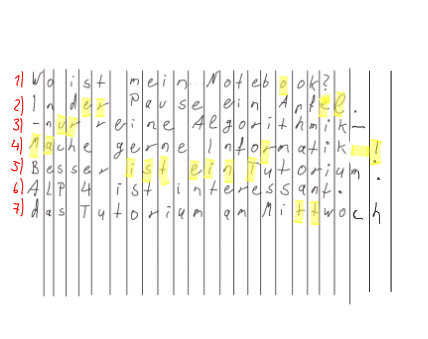
\includegraphics{picture_a4.png}

Ergebnis dieser Abfolge ist der Satz: ``Maurer ist ein Trottel !''

\bibliographystyle{agsm}
\bibliography{alp_IV}

\end{document}



